\documentclass{article}
\usepackage[left=3cm, right=3cm]{geometry}
\usepackage{amsmath}
\usepackage{amssymb}
\usepackage{amsthm}
\usepackage{xcolor}
\usepackage{graphicx}
\usepackage{mathrsfs}
\usepackage{hyperref}
\usepackage{algorithm}
\usepackage{algpseudocode}
\usepackage{booktabs}
\usepackage{threeparttable}

\newcommand{\todo}[1]{[\colorbox{red}{TO-DO:} #1]}
\newcommand{\argmin}[1]{\underset{{#1}}{\mathrm{argmin}\;}}
\newcommand{\dee}{\;\mathrm{d}}
\newcommand{\R}{\mathbb{R}}
\newcommand{\Natural}{\mathbb{N}}

\newtheorem{defn}{Definition}
\newtheorem{remark}{Remark}
\newtheorem{theorem}{Theorem}

\author{Jacob Hauck}
\title{Math 5001 Final Project}


\begin{document}
	\maketitle
	
	\begin{figure}
		\begin{center}
			\includegraphics[width=\textwidth]{MRI_PET_Comparison.png}
		\end{center}
		\caption{A comparison of MRI and PET images of the same person's brain. The bottom two rows show overlays of the images before and after registration. From Goshtasby's book on image registration \cite{goshtasby2005}.}\label{fig:mri_pet_comparison}
	\end{figure}

	\section{Image Registration}

	A patient has an organ scanned. A few months later, the same patient has the same organ scanned. It is of medical importance to determine what has changed in the organ between the two scans, which were performed at different times, from different angles, and possibly using different modalities. This is a typical example of an \textit{image registration} problem.
	
	The images may differ (1) in geometry (for example, the shape of the object in the image) and (2) in  visual features (for example, colors and textures). Imaging an object with the \textit{same} camera from two \textit{different} positions will capture different geometry. On the other hand, imaging an object with \textit{different} cameras from the \textit{same} position will capture the same geometry but possibly different visual features (if, say, one camera took black and white pictures, and the other, color pictures).
	
	To make a reliable comparison of two different images of the same object, we need to ``factor out'' differences caused by the imaging process so that only differences in the underlying object remain. This is essentially the definition of image registration.
	
 	In medical imaging the goal is usually to factor out only geometric differences because differences in visual features may be of importance; some imaging modalities capture complementary visual features, so factoring out these differences might destroy important diagnostic information.
	
	Many techniques focus on the simpler case in which visual features are the same (for example, registering two CT scans); in this case, the problem consists of identifying the geometrical transformation between the two images, which is often a matter of pattern matching. If the two images have very different visual features, then the problem is more challenging; it becomes necessary to rely on the specific kinds of features present in the distribution of images being studied. For example, an algorithm that could register MRI and X-ray CT images might not be able to register ultrasound and PET images without some kind of modification to address the different kinds of features produced by these modalities.
	
	\subsection{Definitions and terms}
	Before we can properly define image registration we need to define an image. There are two perspectives on this: the idealized notion of an image as a function on \([0,1]^n\) (a ``continuous'' image), and the notion of an image as a discrete set of samples of a continuous image.
	
	\newcommand{\unitcube}[1][n]{{[0,1]^{#1}}}
	\newcommand{\contim}[2]{{C\left(#1, #2\right)}}
	\newcommand{\discim}[3]{{D\left(#1, #2; #3\right)}}
	\begin{defn}\label{def:image}
		Let \(n, c \in \Natural\) and \(s \in \Natural^n\).
		\begin{itemize}
			\item An \(n\)\textbf{-dimensional continuous image} with \(c\) \textbf{channels} is a function \(f: \unitcube \to \R^c\). Let
			\begin{equation}\label{eq:cont_im_space}
				\contim{n}{c} = \{\textnormal{all }n\textnormal{-dimensional continuous images with }c\textnormal{ channels}\}
			\end{equation}
			
			\item An \(n\)\textbf{-dimensional discrete image} with \(c\) \textbf{channels} and \textbf{shape} \(s\) is a function \(F: \Natural_0^s \to \R^c\), where 
			\begin{equation*}
				\Natural_0^s := \{i \in (\Natural \cup \{0\})^n \mid i < s\}
			\end{equation*}
			Note that the \(<\) above is taken in the sense of multi-index \(<\). Let
			\begin{equation}\label{eq:disc_im_space}
				\discim{n}{c}{s} = \{\textnormal{all }n\textnormal{-dimensional discrete images with }c\textnormal{ channels and shape }s\}
			\end{equation}
		\end{itemize}
	\end{defn}
	
	We will use lower case letters for continuous images (\(f\)) and parentheses to get their values (\(f(x)\)). Likewise, we will use upper case letters for discrete images (\(F\)) and square brackets to get their values (\(F[i]\)). 
	
	Continuous images are easier to work with theoretically, but discrete images are a practical necessity. Therefore, we would like to relate the two. We do so by the following mapping.
	\newcommand{\grid}{\mathscr{G}}
	\begin{defn}\label{def:sampling_grid}
		Let \(s \in \Natural^n\), and define the \textbf{sampling grid} function \(\grid_s: \Natural_0^s \to [0,1]^n\) by
		\begin{equation}\label{eq:sampling_grid}
			\grid_s(i) = \left(\frac{i_1 + \frac{1}{2}}{s_1}, \frac{i_2 + \frac{1}{2}}{s_2}, \dots, \frac{i_n + \frac{1}{2}}{s_n}\right)
		\end{equation} 
	\end{defn}

	With this definition, we can immediately interpret the samples of an image \(f \in \contim{n}{c}\) as a discrete image \(F \in \discim{n}{c}{s}\) with this definition
	\begin{equation}\label{eq:idealized_to_discrete}
		F[i] = f(\grid_s(i))
	\end{equation}
	We would like to do this in the opposite direction as well, that is, interpret a discrete image as a continuous image, but there are many ways to do this because of the ``gaps'' in discrete images. In other words, we can't invert (\ref{eq:idealized_to_discrete}) because the grid sampling function is not onto. To address this issue, we introduce the notion of \textit{interpolation}.
	\newcommand{\kernel}{\mathcal{K}}
	\begin{defn}\label{def:interpolation}
		Given an \textbf{interpolation kernel} function \(\kernel: \Natural_0^s \times \unitcube \to \R\), the \textbf{interpolation} (by \(\kernel\)) of a discrete image \(F\) with shape \(s\) is the image \(f\) defined by
		\begin{equation}\label{eq:interpolation}
			f(x) = \sum_{i \in \Natural_0^s} F[i]\kernel(i, x)
		\end{equation}
	\end{defn}
	We will use parentheses on an image to get the value of its interpolation; thus, the interpolation of \(F \in \discim{n}{c}{s}\) by a kernel \(\kernel\) at a point \(x\in \unitcube\) is written \(F_\kernel(x)\) or simply \(F(x)\), if the specific kernel is understood or arbitrary. Conversely, we can write \(f_s[i]\) or \(f[i]\) to denote \(f(\mathcal{G}_s(i))\).
	
	Given an image \(f\in\contim{n}{c}\) of an object, suppose that we can assign a physical \textit{reference point} (located in the object) to every \(x \in \unitcube\), the domain of the image. Call this mapping the \textit{reference map}, and denote it by \(\mathcal{R}_f\).
	
	\newcommand{\transf}{\mathcal{T}}
	Suppose we have another image \(g \in \contim{n}{c}\) of the same object. Then we get another reference map \(\mathcal{R}_g\). This induces a relation on \(\unitcube\) that relates points with the same reference point under \(\mathcal{R}_f\) and \(\mathcal{R}_g\). Let's assume that this correspondence can be written in terms of a transformation \(\transf: \unitcube\to\unitcube\):
	\begin{equation*}
		\mathcal{R}_f(x) = \mathcal{R}_g(\transf(x))
	\end{equation*}
	If we can find \(\transf\), then we can compute \(g \circ \transf\), which is ``aligned'' with \(f\) in the sense that \(\mathcal{R}_{g\circ\transf} = \mathcal{R}_g\circ\transf = \mathcal{R}_f\). This is what is meant by ``factoring out'' geometrical differences in the images. The critical assumption that \(\mathcal{R}_f\) and \(\mathcal{R}_g\) are related by \(\transf\) makes the problem of image registration possible to solve (otherwise, we would have to deal with the intractable functions \(\mathcal{R}_f\) and \(\mathcal{R}_g\)). Let's now define image registration properly.
	
	\begin{defn}\label{def:image_registration}
		Let \(f,g\in \contim{n}{c}\) be images of the same object with reference maps \(\mathcal{R}_f\) and \(\mathcal{R}_g\). Suppose there is a transformation \(\transf:[0,1]^n \to [0,1]^n\) such that
		\begin{equation}\label{eq:reference_equality}
			\mathcal{R}_f = \mathcal{R}_g \circ \transf
		\end{equation}
		Then \(f\) is called the \textbf{fixed (or reference) image}, and \(g\) is called the \textbf{moving (or sensed) image}, and \(\transf\) is called the \textbf{transformation fuction}. The \textbf{image registration problem} is to determine \(\transf\) given \(f\) and \(g\).
		
		The \textbf{discrete image registration} problem is to determine the transformation function given only the discrete samples of \(f\) and \(g\), that is, discrete images \(F, G \in \discim{n}{c}{s}\) satisfying \(F[i] = f[i]\) and \(G[j] = g[j]\) for all \(i, j \in \Natural_0^s\).
	\end{defn}
	
	\subsection{Traditional approaches to image registration}
	The classical approach to image registration seeks ``matching features'' in the fixed and moving image, then determines a transformation function that makes the matching features coincide \cite{goshtasby2005}.
	
	For example, in the registration of satellite images it is possible to segment bodies of water using thresholding (because water typically appears darker than land). In this case one would use the segmented regions as the features. To find matching features, one might compute transformation-invariant moments of the regions and define matching regions to be those with sufficiently close moments. Finally, one would find a transformation function that minimizes the distance between matching regions in the fixed and moving images.
	
	\newcommand{\cost}{\mathcal{C}}
	In more recent approaches \cite{christensen-johnson}, one defines a \textit{cost function} \(\cost(\transf; f, g)\) that measures how badly a transformation function \(\transf\) registers the moving image \(g\) to the fixed image \(f\)\footnote{All considerations in this section apply to the discrete image registration problem as well (possibly requiring interpolation or discretization).}. Then the registration problem can be rephrased as an optimization problem in which the minimizer of \(\cost\) is the transformation that solves the registration problem. That is,
	\begin{equation}\label{eq:optimization_registration}
		\transf^* = \argmin{\transf \in \Phi} \cost(\transf; f, g)
	\end{equation}
	where \(\Phi\) is a family of candidate transformation functions, and \(\transf^*\) is the transformation that solves the registration problem. Consider the following example of a cost function
	\begin{equation}\label{eq:L2_registration_cost}
		\cost^2(\transf; f, g) = \int_{[0,1]^n}\big|f(x) - g(\transf(x))\big|^2\dee x
	\end{equation}
	This cost function just measures the \(L^2\) distance between \(f\) and \(g\circ \transf\), which would only work well if the images differ only by a transformation -- a more refined cost function would be necessary if the fixed and moving image have significantly different visual features.
	
	Let \(f,g\in \contim{n}{1}\), and extend \(f\) and \(g\) to \(\R^n\) by setting \(f(x) = 0 = g(x)\) for \(x \notin [0,1]^n\). Suppose that \(\Phi\) is the set of affine transformations of \(\R^n\), and let \(\transf(x) = Ax + b\), where \(A = (A_{ij}) \in \R^{n\times n}\), and \(b = (b_i) \in \R^n\). Then we can write the gradient of \(\cost^2\) with respect to \(\transf\) as
	\begin{align}
		\label{eq:grad_A}
		\frac{\partial \cost^2}{\partial A_{ij}} &= 2 \int_{\unitcube} \Big(f(x) - g(Ax + b)\Big)x_j\frac{\partial g}{\partial x_i}(Ax + b) \dee x \\\notag
		\\
		\label{eq:grad_b}
		\frac{\partial \cost^2}{\partial b_i} &= 2 \int_{\unitcube} \Big(f(x) - g(Ax + b)\Big)\frac{\partial g}{\partial x_i}(Ax + b) \dee x
	\end{align}
	If we can compute the integrals approximately, then we can get the approximate gradient of \(\cost^2\) with respect to \(\transf\). This means that we can use gradient descent to generate approximations of the minimizer \(\transf^*\). This type of iterative optimization scheme is typical of traditional approaches to image registration.
	
	\begin{remark}\label{rmk:feature_remark}
		The feature-matching approach to image registration is a special case of the cost function approach, where the cost function \(\cost\) is given by
		\begin{equation}\label{eq:feature_matching_cost}
			\cost(\transf; f, g) = d(\mathcal{F}(f), \mathcal{F}(g \circ \transf))
		\end{equation}
		where \(\mathcal{F}\) is a feature extraction function, and \(d\) is a distance in the space of features. In the satellite imagery example, the feature extractor is the threshold and region-selection process. The distance would be a sum of absolute differences of the invariant moments of corresponding regions.
	\end{remark}
	
	\section{Generative Adversarial Networks}
	\newcommand{\generator}{\mathcal{G}}
	\newcommand{\discriminator}{\mathcal{D}}
	\newcommand{\prob}{\mathbb{P}}
	In some problems an appropriate cost function may be difficult to find, especially when the fixed and moving images have very different visual features. Assuming that examples of properly registered images are available\footnote{This is not an unreasonable assumption since it is desirable to have a set of examples of properly registered images for the statistical evaluation of registration techniques.}, one might hope to infer an appropriate cost function based on the given examples. 
	
	This situation can be made to fit within the \textit{generative adversarial framework}, in which one finds 
	\begin{enumerate}
		\item An approximation \(\generator\) of a function \(\mathfrak{G}\) such that
		\begin{equation*}
			Y \sim \mathfrak{G}(X)
		\end{equation*}
		for random variables \(X\) and \(Y\)
		\item An approximation \(d\) of a distance \(\mathfrak{d}\left(\prob_Y, \prob_{\generator(X)}\right)\) between the distributions \(\prob_Y\) and \(\prob_{\generator(X)}\) of \(Y\) and \(\generator(X)\).
	\end{enumerate}
	
	In the context of image registration, we would choose \(X=(f, g)\), the pair of the fixed and moving images, and \(Y=(f, g, \transf)\), where \(\transf\) is the transformation function for \(f\) and \(g\). Then \(\generator\) would take two unregistered images to a transformation function that approximately solves the registration problem, and the distance \(d\) would approximately measure the quality of the registration across the distribution of images. Note that we choose \(Y = (f, g, \transf)\) instead of \(Y = \transf\) because we are interested in modeling the relationship between \((f,g)\) and \(\transf\); if we chose \(Y = \transf\), we would only be modeling the distribution of \(\transf\) without capturing its relationship to \((f,g)\).
	
	The distance \(d\) approximated by the generative adversarial approach plays a role similar to the cost function from above; however, the cost function is applied to \textit{particular} fixed-moving image pairs whereas the the distance \(d\) is applied to the \textit{distribution} of fixed-moving image pairs and the \textit{distribution} of transformation functions. The generative adversarial approach takes advantage of this important difference to produce an approximate representation of the solution mapping \(f,g \mapsto \transf\). By contrast, in the cost function approach the minimization of the cost function is the approximation of the solution mapping.
	
	The subtle but important benefit of this approach is that it removes the need for \textit{paired} data. In other words, all you need to apply this technique is a sample of registered images and another sample of unregistered images. Because the model learns at the level of distributions, it is not necessary to have corresponding registered images for every sample of unregistered images.
	
	It is worth looking at two realizations of the generative adversarial framework: first, the original Generative Adversarial Network (GAN) framework and second, the successful, modified version called Wasserstein GAN (WGAN).
	
	\subsection{The original GAN formulation}
	Suppose we want to approximate the distribution of a random variable \(Y\). One way to do this is to approximate its probability density function; however, this is not feasible when the \(Y\) is high-dimensional\footnote{That is, nuch greater than 1 or 2 dimensions.}. Instead, we can model the distribution of \(Y\) by finding a function \(\generator\) such that \(\generator(X)\) has approximately the same distribution as \(Y\) for some random variable \(X\) of our choosing.
	
	\newcommand{\jsd}{\mathrm{JS}}
	\newcommand{\kld}{\mathrm{KL}}
	To this end, let's try to find a function \(\generator\) that minimizes some distance between the distribution \(\prob_Y\) of \(Y\) and the distribution \(\prob_{\generator(X)}\) of \(\generator(X)\). The original GAN authors \cite{GAN} choose the Jensen-Shannon divergence, which is defined in terms of the Kullback-Leibler divergence as follows.
	\begin{defn}\label{def:kl_js_divergence}
		Let \(X\) and \(Y\) be random variables with probability density functions \(p_X\) and \(p_Y\) with respect to the measure \(\mu\).
		\begin{itemize}
			\item The \textbf{Kullback-Leibler divergence} (KL divergence) of the distributions \(\prob_X\) and \(\prob_Y\) of \(X\) and \(Y\) is
			\begin{equation}\label{eq:kl_div}
				\kld\left(\prob_X \Vert \prob_Y\right) = \int p_X(z) \log\left(\frac{p_X(z)}{p_Y(z)}\right) \dee \mu(z)
			\end{equation}
			\item Let \(\prob_m = \frac{\prob_X + \prob_Y}{2}\). Then the \textbf{Jensen-Shannon divergence}\footnote{The KL divergence may not be defined for some distributions, but the JS divergence is always defined because we can choose \(\mu = \prob_m\).} (JS divergence) of the distributions \(\prob_X\) and \(\prob_Y\) is
			\begin{equation}\label{eq:js_div}
				\jsd\left(\prob_X, \prob_Y\right) = \frac{1}{2}\kld(\prob_X \Vert\prob_m) + \frac{1}{2}\kld(\prob_Y \Vert \prob_m)
			\end{equation}
		\end{itemize}
	\end{defn}
	The authors of the GAN paper argue that an iterative algorithm that updates \(\generator\) so that \(\jsd\left(\prob_Y, \prob_{\generator(X)}\right)\) decreases should cause \(\prob_{\generator(X)}\) to converge to \(\prob_Y\). Thus, if \(\generator = \generator_\theta\) is a neural network with parameters \(\theta\), then (assuming the network has enough parameters) using gradient descent to update the paremeters of \(\generator_\theta\) should result in \(\generator_\theta(X)\) having roughly the same distribution as \(Y\). In GAN parlance, the neural network \(\generator_\theta\) is known as the \textit{generator}.
	
	That is all good and well, but we want to imagine that we only have access to a random sample from the distribution of \(Y\), which makes computing the JS divergence difficult\footnote{If it wasn't difficult enough without knowing the density of \(Y\).}. To deal with this difficulty, another neural network \(\discriminator_\varphi\) with parameters \(\varphi\) can be used to approximate \(\jsd\left(\prob_X, \prob_{\generator_\theta(X)}\right)\) by minimizing the \textit{GAN loss}, which is carefully designed to involve only expected values of functions of \(X\) and \(Y\), which we can approximate by sample averages.
	
	\newcommand{\lossgan}{\mathscr{L}_{\textnormal{\tiny GAN}}}
	\newcommand{\expect}{\mathbb{E}}
	\begin{defn}\label{def:loss_gan}
		The \textbf{GAN loss} between random variables \(X\) and \(Y\) of a generator \(\generator\) and a discriminator \(\discriminator\) is the function
		\begin{equation}\label{eq:loss_gan}
			\lossgan(\discriminator; \generator) = -\big(\expect[\log (\discriminator(Y))] + \expect[\log(1 - \discriminator(\generator(X)))]\big)
		\end{equation}
	\end{defn}	
	
	\newcommand{\blah}{\,\boldsymbol{\cdot}\,}
	\begin{theorem}\label{thm:discriminator_minimizes_JSD}
		For a fixed generator \(\generator\), if \(\discriminator^*\) is the minimizer of \(\lossgan(\blah; \generator)\), then
		\begin{equation*}
			\jsd\left(\prob_Y, \prob_{\generator(X)}\right) = \log(2) - \frac{1}{2}\lossgan(\discriminator^*; \generator)
		\end{equation*}
	\end{theorem} 
	
	\begin{proof}
		Suppose that \(\discriminator^*\) minimizes \(\lossgan(\,\boldsymbol{\cdot}\,; \generator)\). Then it maximizes
		\begin{align}
			 -\lossgan(\discriminator; \generator) &= \int p_Y(y) \log(\discriminator(y)) \dee \mu(y) + \int p_{\generator(X)}(y) \log(1 - \discriminator(y)) \dee\mu(y) \\
			 \label{eq:negative_loss_gan_integrand}
			 &= \int \big[p_Y(y)\log(\discriminator(y)) + p_{\generator(X)}(y)\log(1-\discriminator(y))\big] \dee \mu(y) 
		\end{align}
		with respect to \(\discriminator\), where \(p_{\generator(X)}\) is the density of \(\generator(X)\) with respect to the measure \(\mu\). It is easy to verify that the function \(h(t) = a\log(t) + b \log(1-t)\) achieves a unique, global maximum for \(t = \frac{a}{a + b}\) for any \(a \ge 0, b \ge 0\) such that \(a + b \ne 0\). Then at each point \(y\) the integrand of (\ref{eq:negative_loss_gan_integrand}) achieves a unique, global maximum when
		\begin{equation*}
			\discriminator(y) = \frac{p_Y(y)}{p_Y(y) + p_{\generator(X)}(y)}, \qquad y \in \mathrm{supp}(p_Y) \cup \,\mathrm{supp}(p_\generator(X))
		\end{equation*}
		(the value of \(\discriminator(y)\) outside of the supports of \(Y\) and \(\generator(X)\) does not affect the value of the integrand). This implies that (almost everywhere)
		\begin{equation*}
			\discriminator^*(y) = \frac{p_Y(y)}{p_Y(y) + p_{\generator(X)}(y)}, \qquad y \in \mathrm{supp}(p_Y) \cup \,\mathrm{supp}(p_\generator(X))
		\end{equation*}
		Therefore,
		\begin{align*}
			-\frac{1}{2}\lossgan(\discriminator^*; \generator) &= \frac{1}{2}\int \left[p_Y(y) \log\left(\frac{p_Y(y)}{p_Y(y) + p_{\generator(X)}(y)}\right) + p_{\generator(X)}(y)\log\left(\frac{p_{\generator(X)}(y)}{p_Y(y) + p_{\generator(X)}(y)}\right)\right]\dee\mu(y)\\\\
			&= \frac{1}{2}\kld\left(\prob_Y \left\Vert \frac{\prob_Y + \prob_{\generator(X)}}{2}\right.\right) + \frac{1}{2}\kld\left(\prob_{\generator(X)} \left\Vert \frac{\prob_Y+ \prob_{\generator(X)}}{2} \right.\right) + \log\left(\frac{1}{2}\right) \\
			&= \jsd\left(\prob_Y, \prob_{\generator(X)}\right) - \log(2)
		\end{align*}
	\end{proof}
	Suppose we have a neural network \(\discriminator_\varphi\) that minimizes \(\lossgan(\discriminator_\varphi; \generator_\theta)\). Then we can train the generator \(\generator_\theta\) to minimize \(-\lossgan(\discriminator_\varphi; \generator_{\theta})\), which by Theorem \ref{thm:discriminator_minimizes_JSD} is equivalent to minimizing \(\jsd\left(\prob_Y, \prob_{\generator(X)}\right)\). In GAN parlance, \(\discriminator_\varphi\) is called the \textit{discriminator}.
	
	If we use gradient descent to minimize \(-\lossgan(\discriminator_\varphi; \generator_\theta)\) with respect to \(\theta\), we notice that the first term \(\expect\left[\log(\discriminator_\varphi(Y))\right]\) does not contribute to the gradient with respect to \(\theta\). Therefore, it is equivalent to minimize
	\newcommand{\lossgangenerator}{\mathscr{L}_{\textnormal{\tiny GAN,G}}}
	\begin{defn}\label{def:gan_generator_loss}
		The \textbf{GAN generator loss} is
		\begin{equation}\label{eq:gan_generator_loss}
			\lossgangenerator(\discriminator; \generator) = \expect\left[\log(1-\discriminator(\generator(X)))\right]
		\end{equation}
	\end{defn}
	
	There is a slight wrinkle at this point: the discriminator \(\discriminator_\varphi\) is only a good approximation of the JS divergence for a \textit{particular} generator, so when we update the generator using gradient descent, we need to retrain the discriminator for the new and slightly different generator. Therefore, we need to use an alternating training algorithm: train the discriminator to optimality, update the generator, train the discriminator to optimality, update the generator, \dots
	
	In practice, it has been observed that early in training the GAN generator loss provides weak gradients. It is equivalent to minimize a different loss that provides larger gradients.
	\newcommand{\logdgangeneratorloss}{\mathscr{L}^{\prime}_{\textnormal{\tiny GAN,G}}}
	\begin{defn}\label{def:log_d_trick}\textnormal{(The \(-\log(D)\) trick)} 
		The \(-\log(D)\) \textbf{trick GAN generator loss} is the loss
		\begin{equation}\label{eq:log_d_trick}
			\logdgangeneratorloss(\discriminator; \generator) = -\expect\left[\log(\discriminator(\generator(X)))\right]
		\end{equation}
	\end{defn}
	The equivalence of the \(-\log(D)\) trick to the true GAN generator loss follows from the fact that both \(-\log(x)\) and \(\log(1-x)\) are decreasing towards a minimum as \(x \in (0,1)\) approaches 1 (see Figure \ref{fig:log_d_trick}). The trick is effective because the value \(x = \discriminator(\generator(X))\) produced by the discriminator early in training is usually very small because the generator is bad; when \(x\) is small, the gradient of \(\log(1-x)\) is small, but the gradient of \(-\log(x)\) is large.
	\begin{figure}
		\begin{center}
			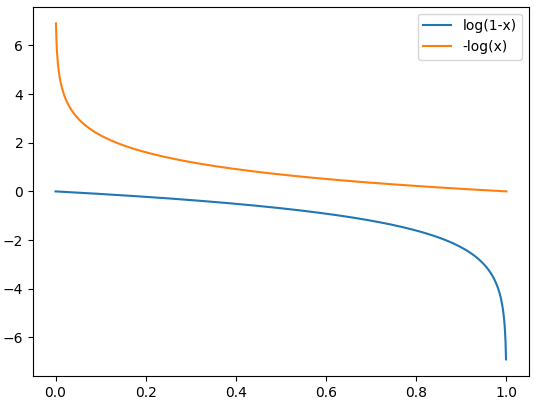
\includegraphics[width=0.8\textwidth]{log_d_trick.png}
		\end{center}
		\caption{Comparison of \(\log(1-x)\) and \(-\log(x)\). Note that when \(x\) is close to 0 the function \(\log(1-x)\) has a small slope, but \(-\log(x)\) has a large slope. This helps improve training of the generator early.}\label{fig:log_d_trick}
	\end{figure}
	
	Finally, if we use sample averages to approximate the various loss functions, we arrive at the GAN training algorithm (Algorithm \ref{alg:gan_training}).

	\newcommand{\approxlossgan}{\widehat{\mathscr{L}}_{\textnormal{\tiny GAN}}}
	\newcommand{\approxlossgangenerator}{\widehat{\mathscr{L}'}_{\textnormal{\tiny GAN,G}}}
	\begin{algorithm}
		\caption{Stochastic Gradient Descent GAN Training Algorithm}\label{alg:gan_training}
		\begin{algorithmic}
			\State Initialize neural networks \(\discriminator_\varphi\) and \(\generator_\theta\) with parameters \(\varphi\) and \(\theta\)
			\For{number of training iterations}
				\For{number of discriminator training steps}
					\State \(\left(x_i\right)_{i=1}^m \gets \) random sample minibatch from the distribution of \(X\)
					\State \(\left(y_i\right)_{i=1}^m \gets \) random sample minibatch from the distribution of \(Y\)
					\State Compute the approximate GAN loss
					\begin{equation*}
						\approxlossgan(\discriminator_\varphi; \generator_\theta) = -\frac{1}{m}\sum_{i=1}^m \Big[\log(\discriminator_\varphi(y_i)) + \log(1-\discriminator_\varphi(\generator_\theta(x_i)))\Big]
					\end{equation*}
					\State Use your favorite gradient descent update rule to update \(\varphi\) with the gradient \(\nabla_\varphi\approxlossgan(\discriminator_\varphi; \generator_\theta)\)
				\EndFor
				\State \(\left(x_i\right)_{i=1}^m \gets \) random sample minibatch from the distribution of \(X\)
				\State Compute the approximate GAN generator loss (using the \(-\log(D)\) trick)
				\begin{equation*}
					\approxlossgangenerator(\discriminator_\varphi; \generator_\theta) = -\frac{1}{m}\sum_{i=1}^m\log(\discriminator_\varphi(\generator_\theta(x_i)))
				\end{equation*}
				\State Use your favorite gradient descent update rule to update \(\theta\) with the gradient \(\nabla_\theta\approxlossgangenerator(\discriminator_\varphi; \generator_\theta)\)
			\EndFor
		\end{algorithmic}
	\end{algorithm}
	
	\begin{remark}\label{rmk:gan_remark}
		The GAN algorithm can also be thought of as a zero-sum, two-player game, in which the first player is the generator and the second player is the discriminator. The players compete with opposite goals: the discriminator attempts to discriminate between the true data distribution and the distribution of the generator, and the generator attempts to fool the discriminator. This is the origin of the term Generative Adversarial Network -- the discriminator is the ``adversary'' of the generator in the game. The minimax equilibrium of the game corresponds to when the discriminator and the generator simultaneously minimize their respective losses.
	\end{remark}
	
	\subsection{Wasserstein GAN}
	
	GANs can work very well, but they can also fail very well. For example, I know from experience that changing the learning rates of the discriminator and generator by even a little bit (10\%, say) can make the difference between successful training and catastrophic failure. In general, the training process for GANs is known to be delicate and unstable.
	
	Numerous techniques have been developed to address this extremely undesirable quality, for example, spectral normalization, label smoothing, noise terms, feature matching, and so on\footnote{The \(-\log(D)\) trick counts, as well.}. By far the most effective technique, Wasserstein GAN (WGAN) is based on a more careful mathematical analysis of the GAN training process.
	
	What is happening when we train a GAN? Let's assume that the discriminator is always trained to near optimality. Then the training of the generator produces a sequence of parameters \(\theta_1, \theta_2, \dots \theta_t, \dots\), which correspond to the sequence of distributions \(\prob_{\generator_{\theta_t}(X)}\). We want that \(\prob_{\generator_{\theta_t}(X)} \to \prob_{\generator_{\theta}(X)} \approx \prob_Y\) in JS divergence as \(\theta_t \to \theta\). In other words, we want the map \(\theta \to \prob_{\generator_\theta(X)}\) to be continuous; in fact, if we want to compute the gradient of the JS distance with respect to \(\theta\), then we also want the JS divergence to be differentiable with respect to \(\theta\). Furthermore, we need the gradient with respect to \(\theta\) to be nonzero in order for gradient descent to work.
	
	This is where the problem arises. The JS divergence is actually a very strong distance (in the sense that it induces a strong topology). Roughly speaking, this makes it difficult for sequences to converge and difficult for functions to be continuous. This is thought to be the origin of the GAN training instability.
	
	The best way to see the problem is through some examples. Let \(X\) and \(Y\) both be uniformly distributed on \([0,1]\), and let \(\generator_\theta(x) = x + \theta\) for \(\theta \in \R\). We can compute the JS divergence directly in this case. There are two possibilities to consider. The easier is when \(|\theta|\ge 1\). In this case \(\generator_\theta(X)\) and \(Y\) have disjoint supports. Then the mixture distribution \(\prob_m = \frac{\prob_Y + \prob_{\generator_\theta(X)}}{2}\) is uniform on the union \([0,1]\cup[\theta, \theta + 1]\) of the supports. Therefore
	\begin{align*}
		\kld\left(\prob_Y \Vert \prob_m\right) &= \int_{[0,1]}p_Y(y)\log\left(\frac{p_Y(y)}{p_m(y)}\right)\dee y \\
		&= \int_{[0,1]} \log(2) \dee y = \log(2)
	\end{align*}
	since the density \(p_m\) of the mixture distribution is constant and equal to \(\frac{1}{2}\) on its support. A similar computation shows that \(\kld\left(\left.\prob_{\generator_\theta(X)}\right\Vert \prob_m\right) = \log(2)\). Thus, \(\jsd\left(\prob_Y, \prob_{\generator_\theta(X)}\right) = \log(2)\). Now consider the case when \(|\theta| < 1\). Then the mixture distribution has two parts
	\begin{equation*}
		p_m(y) = \begin{cases}
			\frac{1}{2} & y \in [0,1] \triangle [\theta, \theta + 1] \\
			1 & y \in [0,1] \cap [\theta, \theta + 1]
		\end{cases}
	\end{equation*}
	and we can write the KL divergence
	\begin{align*}
		\kld(\prob_Y\Vert\prob_m) &= \int_{[0,1] \setminus [\theta, \theta + 1]} p_Y(y)\log\left(\frac{p_Y(y)}{p_m(y)}\right) \dee y + \int_{ [0,1] \cap [\theta, \theta + 1]} p_Y(y)\log\left(\frac{p_Y(y)}{p_m(y)}\right) \dee y \\
		&= \int_{ [0,1] \setminus [\theta, \theta + 1]} \log(2) \dee y = \log(2) \cdot \big|[0,1] \setminus[\theta, \theta+1]\big| \\
		&= |\theta|\log(2)
	\end{align*}
	Similarly, we can write
	\begin{align*}
		\kld(\prob_{\generator_{\theta}(X)} \Vert\prob_m) &= \int_{[\theta, \theta+1]\setminus[0,1]}p_{\generator_\theta(X)}(y)\log\left(\frac{p_{\generator_\theta(X)}(y)}{p_m(y)}\right)\dee y + \int_{[0,1] \cap [\theta, \theta + 1]}p_{\generator_\theta(X)}(y)\log\left(\frac{p_{\generator_\theta(X)}(y)}{p_m(y)}\right)\dee y \\
		&= \int_{[\theta, \theta+1]\setminus[0,1]}\log(2) \dee y = \log(2) \cdot \big|[\theta, \theta+1]\setminus[0,1]\big| \\
		&= |\theta| \log(2)
	\end{align*}
	Therefore \(\jsd\left(\prob_Y, \prob_{\generator_\theta(X)}\right) = |\theta|\log(2)\) when \(|\theta| < 1\). Altogether, then
	\begin{equation}\label{eq:jsd_example}
		\jsd\left(\prob_Y, \prob_{\generator_\theta(X)}\right) =
		\begin{cases}
			|\theta| \log(2) & |\theta| < 1 \\
			\log(2) & |\theta| \ge 1
		\end{cases}
	\end{equation}
	We see from (\ref{eq:jsd_example}) that the JS divergence is continuous and almost everywhere differentiable with respect to \(\theta\), but this apparent victory is hollow; if \(|\theta| > 1\), then the gradient is 0 (see Figure \ref{fig:jsd_example}), so gradient descent will fail.
	\begin{figure}
		\begin{center}
			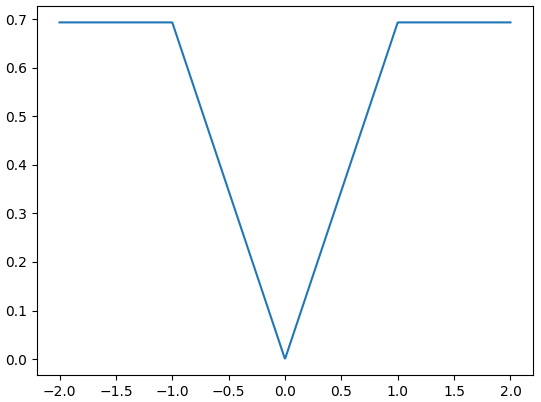
\includegraphics[width=0.7\textwidth]{jsd_example.png}
			\caption{The JS divergence of \(\prob_Y\) and \(\prob_{\generator_\theta(X)}\) as a function of \(\theta\). Note that the gradient descent will succeed in optimizing \(\generator_\theta\) when \(|\theta| < 1\), but it will fail when \(|\theta| > 1\).}
			\label{fig:jsd_example}
		\end{center}
	\end{figure}
	
	In the WGAN paper, the authors give an even more dramatic example. Let \(Z\) be uniformly distributed on \([0,1]\), and let \(Y = X = (0, Z)\). Define \(\generator_\theta(x) = (\theta, x)\). Then
	\begin{equation}\label{eq:jsd_example2}
		\jsd\left(\prob_Y, \prob_{\generator_\theta(X)}\right) = \begin{cases}
			\log(2) & \theta \ne 0 \\
			0 & \theta = 0
		\end{cases}
	\end{equation}
	Now the gradient vanishes everywhere, and gradient descent will always fail to make \(\prob_{\generator_{\theta}(X)}\) converge to \(\prob_Y\), despite the fact that it is obvious by inspection what the optimal value of \(\theta\) is. In fact, as \(\theta_t \to 0\), the JS divergence \(\not\to 0\), so the JS divergence is not even continuous at \(\theta = 0\), the most important value of \(\theta\).
	
	If the JS divergence is too strong, then what is a suitable, weaker distance? The authors of the WGAN paper choose the Wasserstein or earth mover (EM) distance\footnote{Theoretically, the reason that the EM distance is weak (and the motivation for choosing it in the first place) is the fact that it is a metrization of the weak* topology on the space of probability distributions on a compact probability space.}.
	
	\begin{defn}\label{def:wasserstein_dist}
		Given probability distributions \(\prob_X\) and \(\prob_Y\), the Wasserstein or earth mover (EM) distance is defined by
		\begin{equation}\label{eq:wasserstein_dist}
			W(\prob_X, \prob_Y) = \inf_{\gamma \in \Pi(\prob_X, \prob_Y)} \expect_{(x,y) \sim \gamma}\big[|x - y|\big]
		\end{equation}
		where \(\Pi(\prob_X, \prob_Y)\) is the set of all joint distributions whose marginals are \(\prob_X\) and \(\prob_Y\).
	\end{defn}
	In the example from the WGAN paper, the EM distance is just
	\begin{equation}
		W\left(\prob_Y, \prob_{\generator_{\theta}(X)}\right) = |\theta|
	\end{equation}
	Comparing to the JS divergence (\ref{eq:jsd_example2}) we see that the EM distance is continuous and provides a useful gradient for all \(\theta \in \R\), so we should expect gradient descent to work for training a generator. In fact, unlike the JS divergence, the EM distance is always continuous and almost everywhere differentiable:
	
	\begin{theorem}\label{thm:wasserstein_regularity} \cite{WGAN}
		Let \(X\) and \(Y\) be random variables with distributions \(\prob_X\) and \(\prob_Y\), and let \(\prob_{\generator_{\theta}(X)}\) be the distribution of \(\generator_{\theta}(X)\). Then
		\begin{enumerate}
			\item If \(\generator_{\theta}\) is continuous in \(\theta\), then \(W\left(\prob_Y, \prob_{\generator_{\theta}(X)}\right)\) is also continuous in \(\theta\).
			\item If there exists \(L(\theta, x)\) such that
			\begin{gather}
				\label{eq:local_lipschitz}
				\left\lVert \generator_{\theta}(x) - \generator_{\theta'}(x')\right\rVert \le L(\theta, x)(\left\Vert\theta - \theta' \right\rVert + \left\lVert x - x'\right\rVert)
				\quad \text{all } \theta', x'\\\notag\\\label{eq:regularity_assumption1} 
				\expect[L(\theta, X)] < \infty \quad \text{all } \theta
			\end{gather}
			then \(W\left(\prob_Y, \prob_{\generator_{\theta}(X)}\right)\) is continuous everywhere and differentiable almost everywhere.
			\item Statements 1. and 2. are false for the JS divergence.
		\end{enumerate}
	\end{theorem}
	
	It is important to note that \textbf{neural networks} satisfy the hypotheses on \(\generator_{\theta}\) in Theorem \ref{thm:wasserstein_regularity}, statements 1. and 2.
	
	The following theorem completes the argument that the EM distance is the ``right'' distance for GAN training, at least in the sense that it is weaker than JS but still guarantess convergence in distribution.
	
	\begin{theorem}\label{thm:wasserstein_weakness}
		\cite{WGAN}
		Let \(\prob\) be a probability distribution, and let \(\left(\prob_n\right)_{n=1}^\infty\) be a sequence of distributions. If \(\jsd(\prob, \prob_n) \to 0\) as \(n \to\infty\), then \(W(\prob, \prob_n) \to 0\) as \(n\to\infty\). Furthermore, \(\prob_n \overset{\textnormal{dist}}{\to} \prob\) if and only if \(W(\prob, \prob_n)\to 0\).
	\end{theorem}

	So the EM distance is a better choice than the JS divergence. In order to use the EM distance, we need to devise a new GAN loss so that the discriminator approximates the EM distance instead of the JS divergence. Furthermore, we need this new loss to be expressible in terms of expected values so that we can approximate it with sample averages, as we did in the original GAN. This is actually fairly simple due to the following fact (a result of Kantorovich-Rubinstein duality).
	
	\begin{theorem}\label{thm:wasserstein_duality}
		\cite{WGAN}
		Let \(\prob_X\) and \(\prob_Y\) be the distributions of random variables \(X\) and \(Y\). Let \(K > 0\). Then the EM distance
		\begin{equation}\label{eq:wasserstein_duality}
			W(\prob_Y, \prob_X) = \frac{1}{K}\sup_{\lVert h \rVert_L \le K} \big[\expect[h(Y)] - \expect[h(X)]\big]
		\end{equation}
		where the supremum is taken over all real, \(K\)-Lipschitz functions \(h\) on the probability space of \(X\) and \(Y\).
	\end{theorem}
	
	If we use a class of neural networks to approximate the set of all \(K\)-Lipschitz functions, then we can approximate the EM distance up to some unknown and irrelevant factor \(K\) by training the network to solve the maximization problem in (\ref{eq:wasserstein_duality}). This is equivalent to minimizing the WGAN loss:
	\newcommand{\losswgan}{\mathscr{L}_{\textnormal{\tiny WGAN}}}
	\begin{defn}\label{def:wgan_loss}
		Given a discriminator \(\discriminator\) and a generator \(\generator\), the \textbf{WGAN loss} is
		\begin{equation}\label{eq:wgan_loss}
			\losswgan(\discriminator; \generator) = \expect\big[\discriminator(\generator(X))\big] - \expect\big[\discriminator(Y)\big]
		\end{equation}
	\end{defn}
	Suppose we have a neural network \(\discriminator_\varphi\) that minimizes \(\losswgan\); then, just like we did with the original GAN, we can train the generator \(\generator_{\theta}\) to minimize \(-\losswgan(\discriminator_\varphi; \generator_{\theta})\), which by Theorem \ref{thm:wasserstein_duality} is equivalent to minimizing \(W\left(\prob_Y, \prob_{\generator_{\theta}(X)}\right)\).
	
	The biggest difference from the original GAN algorithm is that we must somehow ensure that the network \(\discriminator_\varphi\) is \(K\)-Lipschitz for some \(K\). The authors of the WGAN paper suggest weight clipping, that is, after each gradient descent update to \(\varphi \in \R^\ell\), clip \(\varphi\) to the box \([-c,c]^{\ell}\), where \(c\) is some small, positive constant (a new hyperparameter in the WGAN framework).
	
	If we use gradient descent to minimize \(-\losswgan(\discriminator_\varphi; \generator_\theta)\) with respect to \(\theta\), we notice that the second term \(- \expect\big[\discriminator(Y)\big]\) does not contribute to the gradient with respect to \(\theta\). Therefore, it is equivalent to minimize
	\newcommand{\losswgangenerator}{\mathscr{L}_{\textnormal{\tiny WGAN,G}}}
	\begin{defn}\label{def:wgan_generator_loss}
		Given a discriminator \(\discriminator\) and a generator \(\generator\), the \textbf{WGAN generator loss} is
		\begin{equation}\label{eq:wgan_generator_loss}
			\losswgangenerator(\discriminator, \generator) = -\expect\big[\discriminator(\generator(X))\big]
		\end{equation}
	\end{defn}
	
	As in the original GAN, we can approximate the expected values by sample averages, which leads to the WGAN algorithm (Algorithm \ref{alg:wgan_algorithm}). The WGAN algorithm has enjoyed great empirical success, effectively curing the instability of the original GAN algorithm.
	
	\newcommand{\approxlosswgan}{\widehat{\mathscr{L}}_{\textnormal{\tiny WGAN}}}
	\newcommand{\approxlosswgangenerator}{\widehat{\mathscr{L}}_{\textnormal{\tiny WGAN,G}}}
	\begin{algorithm}
		\caption{Stochastic Gradient Descent WGAN Training Algorithm}\label{alg:wgan_algorithm}
		\begin{algorithmic}
			\State Initialize neural networks \(\discriminator_\varphi\) and \(\generator_\theta\) with parameters \(\varphi\) and \(\theta\)
			\State Fix a clipping parameter \(c > 0\)
			\For{number of training iterations}
				\For{number of discriminator training steps}
					\State \(\left(x_i\right)_{i=1}^m \gets \) random sample minibatch from the distribution of \(X\)
					\State \(\left(y_i\right)_{i=1}^m \gets \) random sample minibatch from the distribution of \(Y\)
					\State Compute the approximate WGAN loss
					\begin{equation*}
						\approxlosswgan(\discriminator_\varphi; \generator_\theta) = \frac{1}{m}\sum_{i=1}^m \Big[\discriminator_\varphi(\generator_{\theta}(x_i)) - \discriminator_\varphi(y_i)\Big]
					\end{equation*}
					\State Use a gradient descent update rule* to update \(\varphi\) with the gradient \(\nabla_\varphi\approxlosswgan(\discriminator_\varphi; \generator_\theta)\)
					\State Clip the parameter \(\varphi\) to the box \([-c, c]^{\ell}\)
				\EndFor
				\State \(\left(x_i\right)_{i=1}^m \gets \) random sample minibatch from the distribution of \(X\)
				\State Compute the approximate WGAN generator loss
				\begin{equation*}
					\approxlosswgangenerator(\discriminator_\varphi; \generator_\theta) = -\frac{1}{m}\sum_{i=1}^m\discriminator_\varphi(\generator_{\theta}(x_i))
				\end{equation*}
				\State Use a gradient descent update rule* to update \(\theta\) with the gradient \(\nabla_\theta\approxlosswgangenerator(\discriminator_\varphi; \generator_\theta)\)
			\EndFor
			\State
			\State * The gradient descent update rule should \textbf{not} use momentum. The authors of the original paper note that training can become unstable when using momentum-based rules.
		\end{algorithmic}
	\end{algorithm}

	\section{Adversarial Image Registration}\label{sec:air}
	When the visual features of two images are very different, it is difficult to design a cost function to register them. Yan \textit{et al.} \cite{yan-xu-rastinehad-wood} study one such case, involving the registration of MRI and ultrasound images. They attempt to overcome the differences in visual features by applying a WGAN in a manner similar to what was described at the beginning of section 2, but with one important difference (other than the insignificant change to discrete images).
	
	As in section 2, let \(X = (F, G)\) be a random pair of fixed and moving discrete images and \(\transf\) the transformation function that registers them. Instead of setting \(Y = (F, G, \transf)\), Yan, \textit{et al.} set \(Y = (F, G \circ \transf)\), where \(G \circ \transf\) is defined by interpreting \(G\) as continuous through interpolation\footnote{More on this in \ref{sec:spatialtransformer}.}. The benefit of this trick is that it allows the discriminator to classify whether images are registered instead of having to learn, independently of the generator, whether the transformation function \(\transf\) registers the images \(F, G\). This is an easier task for convolutional networks, which excel at classification.
	
	We will construct neural networks \(\discriminator_\varphi\) and \(\generator_\theta\) as the WGAN generator and discriminator. Since \(F\) and \(G\) are given, we will define the generator in two steps. The first step takes the images \(F\) and \(G\) and computes an approximate transformation function \(\widehat{\transf}\). The second step computes \(\left(F, G\circ\widehat{\transf}\right)\). If \(\generator_\theta\) is to be a neural network, then it cannot return anything but a vector, so in order to interpret its output as a transformation, we need some parameterization of a family of transformations. Let \(\transf(\lambda)\) denote the transformation corresponding to a parameter \(\lambda \in \R^t\) (this notation emphasizes the dependence of \(\transf\) on \(\lambda\)). Then we want to make the output of the first step of \(\generator_\theta\) a vector in \(\R^t\). We will define the family of transformations being used later.
	
	The WGAN algorithm (Algorithm \ref{alg:wgan_algorithm}) takes care of the training of the neural networks \(\discriminator_\varphi\) and \(\generator_{\theta}\). All that is left is to specify the structure of these networks as they are defined by Yan, \textit{et al.}
	
	\subsection{Convolutional architecture}\label{sec:convolutions}
	The networks we will use for \(\discriminator_\varphi\) and \(\generator_\theta\) will be fairly simple convolutional neural networks. We now define what a convolutional network is, but only in the discrete case, as the network will actually be applied to discrete images. Instead of giving the usual discrete convolution definition, I will give a more general ``machine learning'' version, which includes a bias term  as well as striding, dilation, and centering.
	
	\newcommand{\inchannels}{{C_{\textnormal{in}}}}
	\newcommand{\outchannels}{{C_{\textnormal{out}}}}
	\newcommand{\conv}{\mathrm{conv}}
	\begin{defn}\label{def:discrete_conv}
		Let \((k_H, k_W) \in \Natural^2\), \(\inchannels, \outchannels \in \Natural\).
		\begin{itemize} 
			\item If \(W_c \in \discim{2}{\inchannels}{(k_H, k_W)}\) for \(c=1\) to \(\outchannels\), and \(b \in \R^\outchannels\), then \(\Theta = \left(\left(W_i\right)_{c=1}^{\outchannels}, b\right)\) is called a \textbf{convolution parameter} with \textbf{kernel size} \(k = (k_H, k_W)\), \textbf{input channels} \(\inchannels\), and \textbf{output channels} \(\outchannels\). The images \(W = \left(W_c\right)_{c=1}^\outchannels\) are called the \textbf{weights}, and the vector \(b\) is called the \textbf{bias}.
			
			\item The \textbf{discrete 2D convolution} with parameter \(\Theta\), \textbf{stride} \(\sigma \in \Natural^2\), and \textbf{dilation} \(d \in \Natural^2\) \textbf{centered at} \(o \in \Natural_0^k\) is the function \(\conv_\Theta\) taking a discrete image \(F \in \discim{2}{\inchannels}{s}\) to the discrete image \(G \in \discim{2}{\outchannels}{s'}\) defined by
			\begin{equation}\label{eq:discrete_conv}
				G[i]_c = b_c + \sum_{j \in \Natural_0^k}W_c[j] \cdot F[\sigma i - d(j - o)] \qquad i \in \Natural_0^{s'},\; c =1 \text{ to } \outchannels
			\end{equation}
			where we set \(F[\ell] := 0\) when \(\ell \notin \Natural_0^s\), and \(s' = \left(\left\lfloor \frac{s_1}{\sigma_1}\right\rfloor, \left\lfloor\frac{s_2}{\sigma_2}\right\rfloor\right)\). The symbol \(\sigma i\) means \((\sigma_1 i_1, \sigma_2 i_2)\); a similar definition holds for \(d(j-o)\). We will always choose the center \(o = \left(\left\lfloor \frac{k_H}{2}\right\rfloor, \left\lfloor\frac{k_W}{2} \right\rfloor\right)\).
		\end{itemize}
	\end{defn}

	Intuitively, one can think of a convolution as sliding the weights \(W\) over the input image \(F\). Stride determines how ``quickly'' \(W\) slides over \(F\); if \(\sigma=(2,2)\), then the weights slide two pixels at a time, which should result in an output image that has half the resolution of the input. The dilation effectively ``spreads out'' the weights as they slide; if \(d = (2, 2)\), then the weights are spaced by two pixels as they slide instead of one\footnote{One can also view the image as sliding over the weights, in which case the dilation controls how ``quickly'' the image slides, exactly analogous to the stride.} (see \href{https://ezyang.github.io/convolution-visualizer/}{this} nice animated visualization\footnote{\url{https://ezyang.github.io/convolution-visualizer/}}).
	
	\newcommand{\sigmoid}{\mathfrak{s}}
	\newcommand{\relu}{\mathfrak{r}}
	\begin{defn}\label{def:activation_functions}
		Define the \textbf{activation functions} (which map \(\R \to \R\)).
		\begin{enumerate}
			\item The sigmoid function \(\sigmoid\) defined by
			\begin{equation}
				\label{eq:sigmoid}
				\sigmoid(x) = \frac{1}{1 + e^{-x}}
			\end{equation}
			\item The ReLU function \(\relu\) defined by
			\begin{equation}
				\label{eq:relu}
				\relu(x) = \begin{cases}
					x & x \ge 0 \\
					0 & x < 0
				\end{cases}
			\end{equation}
		\end{enumerate}
		We will apply these functions \textbf{componentwise} to a discrete image \(F\) in the sense that
		\(\sigmoid(F)\) is the discrete image defined by \(\sigmoid(F)[i] = \sigmoid(F[i])\) for all indices \(i\) into \(F\).
	\end{defn}

	It has been found empirically that \textit{residual learning} can improve the performance of deep convolutional neural networks \cite{ResNet}. The idea behind residual learning is to reparameterize the operations of the network as perturbations of the identity\footnote{This is thought to stabilize training by making it easy to learn identity mappings. Previous work had shown that very deep networks performed more poorly than shallower ones despite having greater capacity; by making the identity the ``default'' for each layer, residual learning ensures that a very deep network can't perform any worse than a shallower one.}. To this end, we define the \textit{residual convolution block}.
	\newcommand{\resconv}{\mathrm{resconv}}
	\begin{defn}\label{def:resconv}
		Given convolution parameters \(\Theta_1, \Theta_2, \dots, \Theta_L\) and an activation function \(\rho\), the \textbf{2D residual convolution block} is the function \(\resconv_\rho(\Theta_1, \Theta_2, \dots, \Theta_L)\), which acts on an image \(F \in \discim{2}{\inchannels}{s}\) by
		\begin{equation}
			\resconv_\rho(\Theta_1, \Theta_2, \dots, \Theta_L)(F) = \left[\conv_{\Theta_1} \circ \rho \circ \conv_{\Theta_2} \circ \rho \circ \dots \circ \conv_{\Theta_L}\right](F) + F
		\end{equation}
	\end{defn}
	
	\newcommand{\dweight}{\Theta_\discriminator}
	\newcommand{\gweight}{\Theta_\generator}
	\newcommand{\xweight}{\Theta_\mathcal{X}}
	Now we are ready to define the networks \(\discriminator_\varphi\) and \(\generator_\theta\). Both networks will involve 7 convolutions. Let \(\dweight = \left(\dweight^\ell\right)_{\ell=1}^7\) and \(\gweight = \left(\gweight^\ell\right)_{\ell=1}^7\) be the parameters of these convolutions for the discriminator and generator networks. The kernel sizes, channels, strides and dilations of these convolutions are summarized in Table \ref{table:convolutional_architecture}. Note that both the discriminator and generator convolutions use the same architecture parameters (kernel size, channels, stride, and dilation). 
	
	\begin{table}[t]
		\begin{center}
			\begin{tabular}{@{}lllll@{}}
				\toprule
				\(\ell\) (Layer) & \(k\) (Kernel size) & \(\outchannels\) (Channels) & \(\sigma\) (Stride) &  \(d\) (Dilation) \\
				\midrule
				1 & (3, 3) & 128 & (1, 1) & \textbf{(2, 2)} \\
				2 & (3, 3) & 128 & \textbf{(2, 2)} & (1, 1) \\
				3 & (3, 3) & 128 & \textbf{(2, 2)} & (1, 1) \\
				4 & (3, 3) & 128 & (1, 1) & (1, 1) \\
				5 & (3, 3) & 128 & (1, 1) & (1, 1) \\
				6 & (3, 3) & 128 & (1, 1) & (1, 1) \\
				7 & \textbf{(1, 1)} & \textbf{8} & (1, 1) & (1, 1) \\
				\bottomrule
			\end{tabular}
		\end{center}
		\caption{The architecture parameters of the convolutional layers of \(\discriminator_\varphi\) and \(\generator_\theta\).}
		\label{table:convolutional_architecture}
	\end{table}
	
	Then we define the convolutional subnetwork
	\newcommand{\cat}{\mathrm{cat}}
	\begin{align}\label{eq:conv_network}
		C_\mathcal{X}(F, G) = \big[\relu \circ\conv_{\xweight^7} \circ \relu \circ \resconv_\relu\left(\xweight^4, \xweight^5, \xweight^6\right) \circ \relu \circ \conv_{\xweight^3} \circ \relu \circ \conv_{\xweight^2} \circ \relu \circ \conv_{\xweight^1}\big] (\cat(F, G))
	\end{align}
	where \(\mathcal{X}\) stands for either \(\discriminator\) or \(\generator\), and \(\cat\) is the concatenation function that takes images \(F \in \discim{n}{c_F}{s}\) and \(G \in \discim{n}{c_G}{s}\) to the image \(\cat(F, G) \in \discim{n}{c_F + c_G}{s}\) defined by concatenating the tuple \(G[i]\) to \(F[i]\) to get \(\cat(F,G)[i]\) for all \(i \in \Natural_0^s\).
	
	Suppose the output \(C_\mathcal{X}(F, G) \in \discim{2}{8}{(H, W)}\) for some \(H, W\) that depend on the shape \(s\) of \(F\) and \(G\). If we ``flatten'' the output of \(C_\mathcal{X}(F,G)\) into a vector \(c_\mathcal{X}(F,G) \in \R^{8\cdot W\cdot H}\), then we can apply a fully-connected neural network to this vector to get a final output with the right number of dimensions. For the discriminator Yan, \textit{et al.} use the network
	\newcommand{\FC}{\mathrm{H}}
	\begin{equation}\label{eq:FC_disc}
		\FC_\discriminator(x) = \sigmoid\left(W_\discriminator^2\relu \left(W_\discriminator^1x + b_\discriminator^1\right) + b_\discriminator^2\right)
	\end{equation}
	and for the generator they use
	\begin{equation}\label{eq:FC_gen}
		\FC_\generator(x) = W_\generator^2\relu \left(W_\generator^1x + b_\generator^1\right) + b_\generator^2
	\end{equation}
	where \(x \in \R^{8\cdot W \cdot H}\), the first layer in both networks has 256 hidden units, the second and final layer in \(\FC_\discriminator\) has one unit (recall that a WGAN discriminator should be a real function of its input), and the second and final layer of \(\FC_\generator\) has \(t\) units (recall that our transformations are going to be parameterized by \(\R^t\)).
	
	Bringing this all together, we can define
	\newcommand{\flatten}{\textnormal{flat }}
	\begin{align}
		\discriminator_\varphi(F, G) &= \FC_\discriminator\big(\flatten C_\discriminator(F, G)\big) &&\varphi = \left(\Theta_\discriminator, W_\discriminator^1, W_\discriminator^2, b_\discriminator^1, b_\discriminator^2\right)\\
		\generator_\theta(F, G) &= \Big(F, G \circ \mathcal{T}\big(\FC_\generator\big(\flatten C_\generator(F, G)\big)\big)\Big) &&\theta = \left(\Theta_\generator, W_\generator^1, W_\generator^2, b_\generator^1, b_\generator^2\right)
	\end{align}
	where \(\flatten\)refers to the flattening operation described above, and \(\transf(\lambda)\) is the transformation corresponding to the transformation parameter \(\lambda \in \R^t\).	

	\subsection{Spatial transformers}\label{sec:spatialtransformer}
	We need to propagate gradients through the composition of \(G\) with \(\transf(\lambda)\) in order to use gradient descent to optimize \(\theta\). In machine learning this operation is known as a \textit{spatial transformer} layer \cite{SpatialTransformerNetworks}. As mentioned earlier, we can define this operation by using interpolation on \(G\) to interpret it as a continuous image, composing that continuous image with \(\transf(\lambda)\), then sampling the resulting continuous image to make it discrete again.
	
	\newcommand{\spatialtransf}{\mathcal{S}}
	\begin{defn}\label{def:spatial_transformer}
		Let \(\transf(\lambda)\) be a transformation of \([0,1]^n\) parameterized by \(\lambda \in \R^t\), and let \(r \in \Natural^n\). The \textbf{spatial transformer} with \textbf{grid size} \(r\) adapted to \(\transf(\blah)\) is the function \(\spatialtransf_r(\lambda, \blah)\) defined by
		\begin{equation}\label{eq:spatial_transformer}
			\spatialtransf_r(\lambda, G)[j] = \big(G_\mathcal{K}(\blah) \circ \transf(\lambda)\big)[j] = \sum_{i \in \Natural_0^s}G[i]\mathcal{K}\big(i,\transf(\lambda)\big(\grid_r(j)\big)\big)\qquad j \in \Natural_0^r, G \in \discim{n}{c}{s}
		\end{equation}
		where \(\mathcal{K}\) is an interpolation kernel used to define \(G_\mathcal{K}(\blah)\) (recall Definition \ref{def:interpolation}). Note that \(\spatialtransf_r(\lambda, G) \in \discim{n}{c}{r}\) if \(G \in \discim{n}{c}{s}\)
	\end{defn}
	
	In this definition I have emphasized the dependence of \(\spatialtransf\) on \(\lambda\) because we would like to be able to compute the Jacobian of \(\spatialtransf\) with respect to \(\lambda\) to use gradient descent in a neural network that involves a spatial transformer. Fix \(x\); then \(\lambda \mapsto \transf(\lambda)(x)\) is a function mapping \(\R^t \to \R^n\). Let \(L(\lambda, x)\) be the Jacobian of this function. Then we can write the Jacobian of \(\spatialtransf\) with respect to \(\lambda\) as
	\begin{align}\label{eq:spatial_transformer_jacobian}
		J_{jk}(\lambda, G) = \frac{\partial \spatialtransf[j]}{\partial \lambda_k} &= \sum_{i\in \Natural_0^s} G[i]\frac{\partial\mathcal{K}\left(i,\transf(\lambda)\big(\grid(j)\big)\right)}{\partial \lambda_k}\\ \notag
		&= \sum_{i \in \Natural_0^s} G[i] \nabla\mathcal{K}\left(i, \transf(\lambda)\big(\grid(j)\big)\right)L_{\blah k}(\lambda, x)
	\end{align}
	where \(L_{\blah k}\) is the \(k\)-th column of \(L\). For example, suppose that \(\lambda = (A, b)\), where \(A \in \R^{n\times n}\) and \(b \in \R^n\), and let \(\transf(\lambda)(x) = Ax + b\). First, let's compute \(L_{\blah k}\), where \(k = (\ell, m)\) points to \(A_{\ell m}\). We have \begin{equation*}
		L_{ik} = \frac{\partial(A_{i\blah}x + b_i)}{\partial A_{\ell m}} = x_m\delta_{i\ell}
	\end{equation*}
	where \(\delta\) is the Kronecker delta function, and \(A_{i\blah}\) is the \(i\)-th row of \(A\). So \(L_{\blah k}\) is a vector with \(n\) components, all zero except for component \(\ell\) equal to \(x_m\). Thus, we get the Jacobian with respect to \(A\) of a spatial transformer \(\spatialtransf\) adapted to \(\transf\) via
	\begin{equation*}
		\frac{\partial \spatialtransf[j]}{\partial A_{\ell m}} = \sum_{i \in \Natural_0^s}G[i] \frac{\partial \mathcal{K}}{\partial x_\ell}\left(i, A\grid(j)+b\right) \grid(j)_m
	\end{equation*}
	Second, let's compute \(L_{\blah k}\) when \(k\) points to \(b_k\). Then
	\begin{equation*}
		L_{ik} = \frac{\partial(A_{i \blah} x + b_i)}{\partial b_k} = \delta_{ik}
	\end{equation*}
	Thus, we get the Jacobian
	\begin{equation*}
		\frac{\partial \spatialtransf[j]}{\partial b_k} = \sum_{i \in \Natural_0^s} G[i] \frac{\partial \mathcal{K}}{\partial x_k}(i, A\grid(j) + b)
	\end{equation*}
	Although this is not a common practical choice of interpolation kernel in machine learning, the following choice of \(\mathcal{K}\) is nice for the purposes of this example. Let's use the Gaussian interpolation kernel
	\begin{equation*}
		\mathcal{K}(i, x) = C\cdot\mathrm{exp}\left(-\frac{|x - \grid(i)|^2}{2\sigma^2}\right)
	\end{equation*}
	for some suitable choice of constants \(C\) and \(\sigma\). Then our Jacobian becomes
	\begin{align*}
		\frac{\partial \spatialtransf[j]}{\partial A_{\ell m}} &= \frac{1}{\sigma^2}\sum_{i \in \Natural_0^s} G[i]\mathcal{K}(i, A\grid(j) + b)\big(\grid(i)_\ell - \grid(j)_\ell\big)\grid(j)_m \\
		\frac{\partial \spatialtransf[j]}{\partial b_k} &=\frac{1}{\sigma^2}\sum_{i \in \Natural_0^s} G[i]\mathcal{K}(i, A\grid(j)+b)\big(\grid(i)_k - \grid(j)_k\big)
	\end{align*}
	At this point, it should be fairly clear how this gradient computation can be carried out numerically (albeit somewhat inefficiently, perhaps). Usually the interpolation kernel is chosen to be either the nearest-neighbor kernel or the bilinear kernel. These kernels have a small support, which limits the number of terms in the summation to a very small number, thereby increasing the efficiency of this operation. There is also the successful Region of Interest Align kernel used in localization and segmentation tasks. It is a somewhat more sophisticated version of the bilinear kernel.
	\section{Experiments}\label{sec:experiments}
	Rather than write this section twice, I have written up the experimental portion of this project in Google Colab, an online service that makes it easy to edit, run, comment and, most importantly, share code\footnote{This isn't a Google advertisement -- Colab has its drawbacks, too.}. You can find the project at this \href{https://colab.research.google.com/drive/1_rf-bgT5ZCrSlfNW0wNB_i82z4Np_rEE?usp=sharing}{link}\footnote{In case clicking on link didn't work: \url{https://colab.research.google.com/drive/1_rf-bgT5ZCrSlfNW0wNB_i82z4Np_rEE?usp=sharing}}, which should give you access to view, run, and edit the code and commentary of the project.
	\pagebreak
	\bibliographystyle{plain}
	\bibliography{References/references.bib}
\end{document}